\Large\textbf{}\\
\Large\textbf{Use Case 1 - Creazione nuovo layout} \\
\vspace{0.5cm}
%\begin{figure}[h]
%  \centering
%  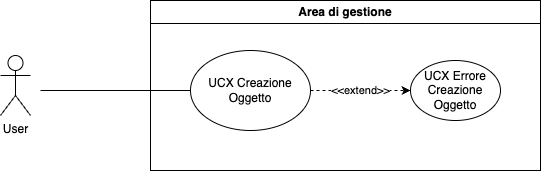
\includegraphics[width=0.8\textwidth]{UseCasesImages/ObjCr.png}
%\end{figure}
\large\textbf{} \\
\textbf{Attori:} User\\
\textbf{Pre-condizione:} Avvio dell'applicazione da parte dell'utente\\
\textbf{Post-condizione: } Creazione del layout magazzino\\
\textbf{Scenario Principale:}  All'utente viene richiesto se caricare un layout esistente o se creare 
un nuovo layout.\\
\vspace{0.5cm}

\Large\textbf{}\\
\Large\textbf{Use Case 1.1 - Creazione Nuovo magazzino} \\
\vspace{0.5cm}
%\begin{figure}[h]
%  \centering
%  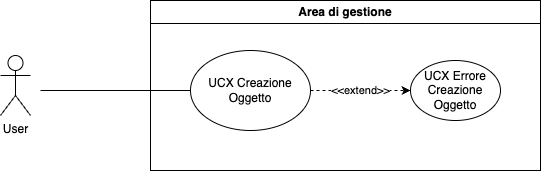
\includegraphics[width=0.8\textwidth]{UseCasesImages/ObjCr.png}
%\end{figure}
\large\textbf{} \\
\textbf{Attori:} User\\
\textbf{Pre-condizione:} E' stata selezionata la modalità: "Creazione manuale magazzino" \\
\textbf{Post-condizione: } Nuovo layout magazzino creato correttamente\\
\textbf{Scenario Principale:}  L'utente viene invitato ad indicare le dimensioni del magazzino in modo da poterne creare il layout.\\
\textbf{Estensioni: } UC1.1.1 - Errore Creazione Layout magazzino\\
\vspace{0.5cm}

\Large\textbf{}\\
\Large\textbf{Use Case 1.2 Importazione layout magazzino} \\
\vspace{0.5cm}
%\begin{figure}[h]
%  \centering
%  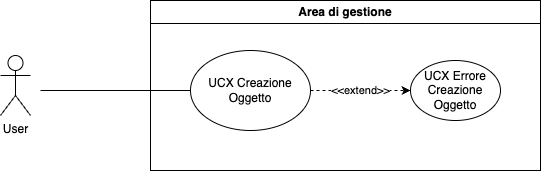
\includegraphics[width=0.8\textwidth]{UseCasesImages/ObjCr.png}
%\end{figure}
\large\textbf{} \\
\textbf{Attori:} User\\
\textbf{Pre-condizione:} E' stato selezionata la modalità: "importazione layout magazzino" \\
\textbf{Post-condizione: } Importazione Layout Magazzino\\
\textbf{Scenario Principale:}  Il magazzino viene correttamente importato da layout esistente.\\
\textbf{Estensioni: } UC1.2.1 - Errore Importazione Layout\\
\vspace{0.5cm}


\Large\textbf{}\\
\Large\textbf{Use Case 2 - Creazione scaffalatura} \\
\vspace{0.5cm}
%\begin{figure}[h]
%  \centering
%  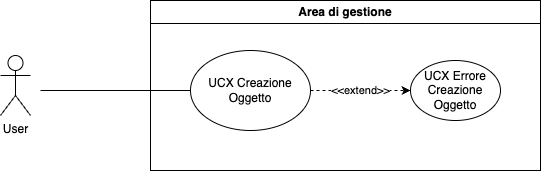
\includegraphics[width=0.8\textwidth]{UseCasesImages/ObjCr.png}
%\end{figure}
\large\textbf{} \\
\textbf{Attori:} User\\
\textbf{Pre-condizione:} Richiesta nuovi inserimento scaffalatura \\
\textbf{Post-condizione: } Creazione corretta della scaffalatura\\
\textbf{Scenario Principale:}  L'utente crea una nuova scaffalatura inserendone le \textit{specifiche caratteristiche}. Se i dati inseriti non rispettano il \textit{criterio prestabilito} viene visualizzato un messaggio di errore.\\
\textbf{Estensioni: } UC2.1 - Errore Creazione scaffalatura\\
\vspace{0.5cm}

\Large\textbf{}\\
\Large\textbf{Use Case 3 - Spostamento scaffalatura} \\
\vspace{0.5cm}
%\begin{figure}[h]
%  \centering
%  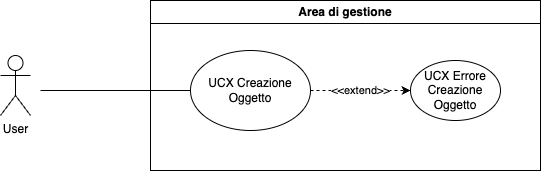
\includegraphics[width=0.8\textwidth]{UseCasesImages/ObjCr.png}
%\end{figure}
\large\textbf{} \\
\textbf{Attori:} User\\
\textbf{Pre-condizione:} Richiesta spostamento scaffalatura \\
\textbf{Post-condizione: } Scaffallatura spostata \\
\textbf{Scenario Principale:}  L'utente selezione la scaffalatura da spostare e il nuovo spazio dove posizionarla.\\
\textbf{Estensioni: } UC3.1 - Errore Spostamento Scaffallatura\\
\vspace{0.5cm}

\Large\textbf{}\\
\Large\textbf{Use Case 4 - Modifica scaffalatura} \\
\vspace{0.5cm}
%\begin{figure}[h]
%  \centering
%  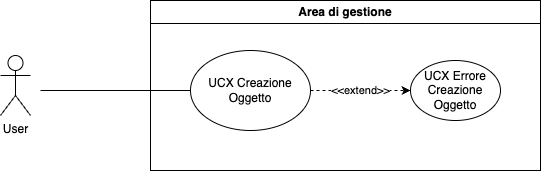
\includegraphics[width=0.8\textwidth]{UseCasesImages/ObjCr.png}
%\end{figure}
\large\textbf{} \\
\textbf{Attori:} User\\
\textbf{Pre-condizione:} Scaffallatura correttamente presente \\
\textbf{Post-condizione: } Corretta modifica scaffalatura\\
\textbf{Scenario Principale:}  L'utente, dopo aver selezionato la scaffalatura, seleziona il comando "Modifica scaffalatura". \\
\textbf{Estensioni: } UC4.1 - Errore modifica scaffalatura\\
\vspace{0.5cm}

\Large\textbf{}\\
\Large\textbf{Use Case 5 - Selezione scaffalatura} \\
\vspace{0.5cm}
%\begin{figure}[h]
%  \centering
%  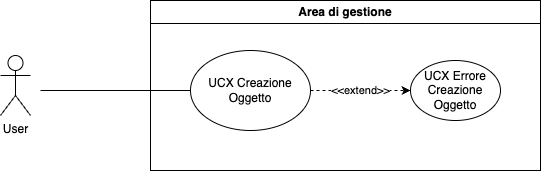
\includegraphics[width=0.8\textwidth]{UseCasesImages/ObjCr.png}
%\end{figure}
\large\textbf{} \\
\textbf{Attori:} User\\
\textbf{Pre-condizione:} Scaffallatura correttamente presente \\
\textbf{Post-condizione: } Visualizzazione dati scaffalatura\\
\textbf{Scenario Principale:}  L'utente sta navigando\textsuperscript{G} all'interno del magazzino e prova a selezionare una scaffalatura esistente. \\
\vspace{0.5cm}
